%% BioMed_Central_Tex_Template_v1.06
%%                                      %
%  bmc_article.tex            ver: 1.06 %
%                                       %

%%IMPORTANT: do not delete the first line of this template
%%It must be present to enable the BMC Submission system to
%%recognise this template!!

%%%%%%%%%%%%%%%%%%%%%%%%%%%%%%%%%%%%%%%%%
%%                                     %%
%%  LaTeX template for BioMed Central  %%
%%     journal article submissions     %%
%%                                     %%
%%          <8 June 2012>              %%
%%                                     %%
%%                                     %%
%%%%%%%%%%%%%%%%%%%%%%%%%%%%%%%%%%%%%%%%%


%%%%%%%%%%%%%%%%%%%%%%%%%%%%%%%%%%%%%%%%%%%%%%%%%%%%%%%%%%%%%%%%%%%%%
%%                                                                 %%
%% For instructions on how to fill out this Tex template           %%
%% document please refer to Readme.html and the instructions for   %%
%% authors page on the biomed central website                      %%
%% http://www.biomedcentral.com/info/authors/                      %%
%%                                                                 %%
%% Please do not use \input{...} to include other tex files.       %%
%% Submit your LaTeX manuscript as one .tex document.              %%
%%                                                                 %%
%% All additional figures and files should be attached             %%
%% separately and not embedded in the \TeX\ document itself.       %%
%%                                                                 %%
%% BioMed Central currently use the MikTex distribution of         %%
%% TeX for Windows) of TeX and LaTeX.  This is available from      %%
%% http://www.miktex.org                                           %%
%%                                                                 %%
%%%%%%%%%%%%%%%%%%%%%%%%%%%%%%%%%%%%%%%%%%%%%%%%%%%%%%%%%%%%%%%%%%%%%

%%% additional documentclass options:
%  [doublespacing]
%  [linenumbers]   - put the line numbers on margins

%%% loading packages, author definitions

\documentclass[twocolumn]{bmcart}% uncomment this for twocolumn layout and comment line below
%\documentclass{bmcart}

%%% Load packages
%\usepackage{amsthm,amsmath}
%\RequirePackage{natbib}
%\RequirePackage[authoryear]{natbib}% uncomment this for author-year bibliography
%\RequirePackage{hyperref}
\usepackage[utf8]{inputenc} %unicode support
%\usepackage[applemac]{inputenc} %applemac support if unicode package fails
%\usepackage[latin1]{inputenc} %UNIX support if unicode package fails
\usepackage{float}
%\usepackage[showframe]{geometry}
\usepackage{lipsum}
%\usepackage{multicols}{2}
%%%%%%%%%%%%%%%%%%%%%%%%%%%%%%%%%%%%%%%%%%%%%%%%%
%%                                             %%
%%  If you wish to display your graphics for   %%
%%  your own use using includegraphic or       %%
%%  includegraphics, then comment out the      %%
%%  following two lines of code.               %%
%%  NB: These line *must* be included when     %%
%%  submitting to BMC.                         %%
%%  All figure files must be submitted as      %%
%%  separate graphics through the BMC          %%
%%  submission process, not included in the    %%
%%  submitted article.                         %%
%%                                             %%
%%%%%%%%%%%%%%%%%%%%%%%%%%%%%%%%%%%%%%%%%%%%%%%%%


\def\includegraphic{}
\def\includegraphics{}
\usepackage{graphicx}



%%% Put your definitions there:
\startlocaldefs
\endlocaldefs


%%% Begin ...
\begin{document}
\begin{multicols}

%%% Start of article front matter
\begin{frontmatter}

\begin{fmbox}
\dochead{Software}

%%%%%%%%%%%%%%%%%%%%%%%%%%%%%%%%%%%%%%%%%%%%%%
%%                                          %%
%% Enter the title of your article here     %%
%%                                          %%
%%%%%%%%%%%%%%%%%%%%%%%%%%%%%%%%%%%%%%%%%%%%%%

\title{SEPIA: Simulation-based Evaluation of Prioritization Algorithms}

%%%%%%%%%%%%%%%%%%%%%%%%%%%%%%%%%%%%%%%%%%%%%%
%%                                          %%
%% Enter the authors here                   %%
%%                                          %%
%% Specify information, if available,       %%
%% in the form:                             %%
%%   <key>={<id1>,<id2>}                    %%
%%   <key>=                                 %%
%% Comment or delete the keys which are     %%
%% not used. Repeat \author command as much %%
%% as required.                             %%
%%                                          %%
%%%%%%%%%%%%%%%%%%%%%%%%%%%%%%%%%%%%%%%%%%%%%%

\author[
   addressref={aff1},
   noteref={n1},
]{\inits{KA}\fnm{Kimberly} \snm{Almaraz}}
\author[
   addressref={aff1},
   noteref={n1},
]{\inits{TJJ}\fnm{Tyler} \snm{Jang}}
\author[
   addressref={aff1},
   noteref={n1},
]{\inits{ML}\fnm{McKenna} \snm{Lewis}}
\author[
   addressref={aff1},
   noteref={n1},
]{\inits{TN}\fnm{Titan} \snm{Ngo}}
\author[
   addressref={aff1},
   noteref={n1},
]{\inits{MS}\fnm{Miranda} \snm{Song}}
\author[
   %addressref={aff1},
   %noteref={n1},
   email={a1moshir@ucsd.edu}
]{\inits{NM}\fnm{Niema} \snm{Moshiri}}
%%%%%%%%%%%%%%%%%%%%%%%%%%%%%%%%%%%%%%%%%%%%%%
%%                                          %%
%% Enter the authors' addresses here        %%
%%                                          %%
%% Repeat \address commands as much as      %%
%% required.                                %%
%%                                          %%
%%%%%%%%%%%%%%%%%%%%%%%%%%%%%%%%%%%%%%%%%%%%%%

\address[id=aff1]{%                           % unique id
  \orgname{Department of Computer Science and Engineering, University of California San Diego}, % university, etc
  \street{9500 Gilman Dr.},                     %
  \postcode{92093}                                % post or zip code
  \city{La Jolla},                              % city
  \cny{USA}                                    % country
}


%%%%%%%%%%%%%%%%%%%%%%%%%%%%%%%%%%%%%%%%%%%%%%
%%                                          %%
%% Enter short notes here                   %%
%%                                          %%
%% Short notes will be after addresses      %%
%% on first page.                           %%
%%                                          %%
%%%%%%%%%%%%%%%%%%%%%%%%%%%%%%%%%%%%%%%%%%%%%%

\begin{artnotes}
%\note{Sample of title note}     % note to the article
\note[id=n1]{Equal contributor} % note, connected to author
\end{artnotes}

%\end{fmbox}% comment this for two column layout

%%%%%%%%%%%%%%%%%%%%%%%%%%%%%%%%%%%%%%%%%%%%%%
%%                                          %%
%% The Abstract begins here                 %%
%%                                          %%
%% Please refer to the Instructions for     %%
%% authors on http://www.biomedcentral.com  %%
%% and include the section headings         %%
%% accordingly for your article type.       %%
%%                                          %%
%%%%%%%%%%%%%%%%%%%%%%%%%%%%%%%%%%%%%%%%%%%%%%

\begin{abstractbox}

\begin{abstract} % abstract
\parttitle{Background}
The ability to prioritize people living with HIV based on the risk of future transmissions could aid public health officials in performing epidemiological intervention. While methods exist to perform such prioritization based on molecular data, their effectiveness is poorly understood, and it is unclear as to how one can directly compare the accuracy of different methods. We introduce SEPIA (Simulation-based Evaluation of PrIoritization Algorithms), a novel simulation-based framework for determining the effectiveness of prioritization methods. Under our several defined metrics, we analyze different variables in the simulated contact and transmission histories to quantify the efficacy of algorithms' results. We use FAVITES, an epidemic simulation tool, to generate this simulated data. We personally used SEPIA to analyze the results of both distance-based and phylogenetic prioritization methods.

\parttitle{Results}
%Text for this section.
Upon testing SEPIA on two different prioritization algorithms, ProACT (phylogenetic) and HIV-Trace (distance), we found that, while ProACT performed slightly better than HIV-TRACE in producing an ordering of individuals by their likelihood of transmitting HIV, the results of both algorithms were close to random. We calculated Kendall Tau-b correlation coefficients for the results of both algorithms in different epidemic conditions, and they consistently had correlation coefficients close to 0.00.

\parttitle{Conclusion}
%Text for this section.
We hope that SEPIA will assist researchers in evaluating the efficacy of newly-developed prioritization tools for HIV in comparing and improving new and existing tools. More accurate tools may be developed in the future with the use of SEPIA.

\end{abstract}

%%%%%%%%%%%%%%%%%%%%%%%%%%%%%%%%%%%%%%%%%%%%%%
%%                                          %%
%% The keywords begin here                  %%
%%                                          %%
%% Put each keyword in separate \kwd{}.     %%
%%                                          %%
%%%%%%%%%%%%%%%%%%%%%%%%%%%%%%%%%%%%%%%%%%%%%%

\begin{keyword}
\kwd{SEPIA}
\kwd{HIV}
\kwd{Prioritization}
\kwd{Metrics}
\kwd{Simulation-based Evaluation}
\kwd{FAVITES}
\kwd{Phylogenetic}
\end{keyword}

% MSC classifications codes, if any
%\begin{keyword}[class=AMS]
%\kwd[Primary ]{}
%\kwd{}
%\kwd[; secondary ]{}
%\end{keyword}

\end{abstractbox}

\end{fmbox}% uncomment this for twocolumn layout

\end{frontmatter}

%%%%%%%%%%%%%%%%%%%%%%%%%%%%%%%%%%%%%%%%%%%%%%
%%                                          %%
%% The Main Body begins here                %%
%%                                          %%
%% Please refer to the instructions for     %%
%% authors on:                              %%
%% http://www.biomedcentral.com/info/authors%%
%% and include the section headings         %%
%% accordingly for your article type.       %%
%%                                          %%
%% See the Results and Discussion section   %%
%% for details on how to create sub-sections%%
%%                                          %%
%% use \cite{...} to cite references        %%
%%  \cite{koon} and                         %%
%%  \cite{oreg,khar,zvai,xjon,schn,pond}    %%
%%  \nocite{smith,marg,hunn,advi,koha,mouse}%%
%%                                          %%
%%%%%%%%%%%%%%%%%%%%%%%%%%%%%%%%%%%%%%%%%%%%%%

%%%%%%%%%%%%%%%%%%%%%%%%% start of article main body
% <put your article body there>

%%%%%%%%%%%%%%%%
%% Background %%
%%
%
%\section*{Content}
%Text and results for this section, as per the individual journal's instructions for authors. %\cite{koon,oreg,khar,zvai,xjon,schn,pond,smith,marg,hunn,advi,koha,mouse}

\section*{Background}
Human immunodeficiency virus (HIV) is one of the world's most deadly infectious diseases, significantly impacting regions including sub-Saharan Africa, Asia, the Pacific, and Latin America \cite{cdc1}. In 2019, there were 38.0 million people living with HIV globally, with 1.7 million people newly infected and 690,000 HIV-related deaths \cite{who}. Methods of epidemic intervention include treatments such as antiretroviral therapy (ART) and awareness programs \cite{cdc2}. Given the scale of the epidemic and the difficulties in tracing viral transmissions, the deployment of limited resources can be optimized using tools that evaluate the transmission of HIV and determine which individuals are most at risk. \cite{wertheim2018growth}.

Analyses of viral sequences are often used to track the evolution and spread of the virus, with each genetic sample representing the specific mutated variants of HIV in each HIV positive individual \cite{wertheim2018growth}. These viral sequences are usually taken from individuals starting ART and seeking treatment at medical facilities. Researchers have developed tools that each take in a list of such sequences and output an ordering that indicates each individual's relative risk of transmitting HIV to others. With inferred data from these tools, health care officials can better determine where to direct epidemiological intervention and resources \cite{wertheim2018growth}.

Existing tools for molecular viral epidemiology that utilize assembled viral genomes collected from patients include HIV-TRACE (CITE POND ET AL PAPER ABOUT HIV-TRACE) and ProACT \cite{moshiri2019ProACT}, and these tools can be used to predict the risk of future transmissions of each sampled individual \cite{wertheim2018growth}. HIV-TRACE and ProACT fundamentally differ in underlying prioritization approach, and the following questions naturally arise: How well does a given tool perform, and which tool is superior in specific contexts? In real epidemics, the ground truth of who infected whom typically does not exist or is error-prone, and as such, there does not exist a standard for measuring the accuracy of molecular epidemiological prioritization techniques.

% TODO - titan read this whole block 
% short summary of sepia, details of how it works in detail should be elsewhere  in the methods section if at all, reword for better grammer
To address this open problem, we introduce our novel framework, Simulation-based Evaluation of PrIoritization Algorithms (SEPIA). SEPIA utilizes simulated epidemic data, such as those generated by FAVITES \cite{moshiri2018favites} or PANGEA.HIV.sim (CITE PANGEA PAPER), in which the ground truth of the entire epidemic is known. Given a prioritization of a simulated dataset, SEPIA will compare the prioritization against the ground truth and compute various metrics of accuracy to assess the performance of the prioritization. The metrics produced by SEPIA can then be used to characterize the performance of a single prioritization approach on different epidemic scenarios (represented by different simulated datasets) as well as to directly compare the performance of multiple prioritization approaches.

SEPIA works by taking in two different data sets. The first data set will come from running a prioritization algorithm and comparing to the metrics producing the order in which individuals are prioritized on. The order in which individuals are prioritized will come from the prioritization tool being evaluated such as HIV-Trace. This first data set comes from running the prioritization tool with the simulated data from FAVITES. The second data set used as an input is the simulated data that. The simulated data will have complete data on what the transmission network, contact network, and phylogenetic tree should be. Using FAVITES as our simulated data is important as there is a full and complete transmission history. We cannot use real data in this instance as real data only contains reported transmissions making that transmission network incomplete. The first thing SEPIA will do is take each person from the simulated data and compare them to the specified metric. This comparison will then output a value for each individual. SEPIA takes in two different simulated data sets: the contact and transmission histories in order to construct an optimal ordering which is determined by our metrics. Each metric has a different method for determining the optimal order in the data set. By comparing this optimal ordering to those produced by prioritization methods, we can quantify the efficacy of different predictive models as a measure of how closely correlated the two orderings are. This framework can be utilized to evaluate the effectiveness of both existing and future prioritization tools.

%Figure 1
\begin{figure}
\centering
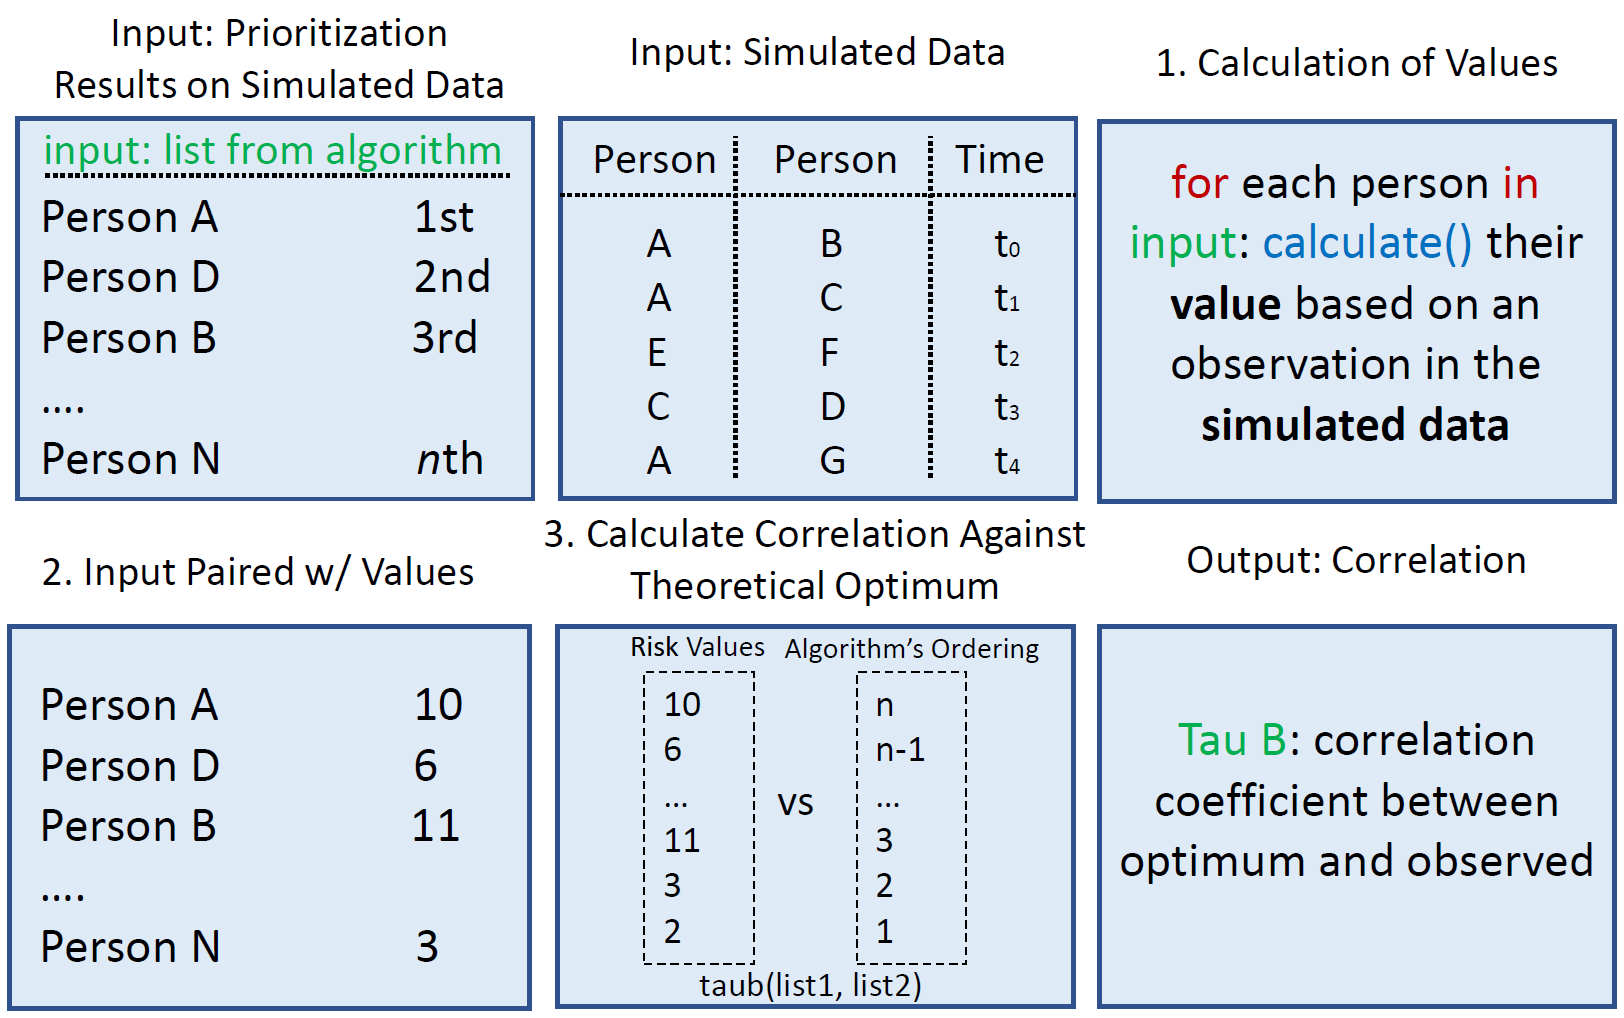
\includegraphics[scale=0.28]{Figures/SEPIA workflow.png}
\caption{This flowchart represents the different stages of SEPIA. The first two boxes indicate the two different inputs that SEPIA will need in order to properly evaluate the algorithms. The simulated data used will be the first input for SEPIA. The second input will be the results on how the individuals are ranked when ran on the prioritization tool. The second input is the list of ranked individuals}
\end{figure}

SEPIA will take two different sets of data for its input. The first input will be the prioritization results ran on simulated data and the  second input will be the simulated data gathered from FAVITES. The first thing SEPIA will do is assign a priority value based off the simulated data. This priority value will then be given a rank determined from the metric that was used. Each person in the data will have a priority value and this value becomes a rank on how much each person should be prioritized. This rank gets compared to the algorithms ordering on how will it prioritizes each person. This comparison is done with the Kendall Tau calculation. When compared SEPIA will output a coefficient between the ranked values and the algorithms ordering.

\section*{Methods}

To construct optimal orderings for evaluating prioritization algorithms, it is necessary to have knowledge of all events within a given time frame. This is captured through the contact history, which represents all interactions between individuals through which HIV could have been transmitted with respective times, as well as the transmission history, which represents all actual occurrences of HIV transmission with respective times. We attempted to use real world data to generate results. However, given the real-world limitations of data collection, it is difficult to know whether any contact and transmission networks assembled from actual data are accurate or complete. Without a true transmission history, we cannot determine a potential optimal ordering of the data set. Thus, simulated data must be utilized to evaluate prioritization algorithms in order to obtain a complete transmission history.

SEPIA utilizes the framework FAVITES (FrAmework for VIral Transmission and Evolution Simulation) for the generation of simulated data that can be used to test prioritization algorithms. FAVITES simulates end-to-end HIV epidemics including the full contact and transmission network(\textit{Figure 2}). FAVITES includes both random processes and user-selected models that holds parameters such as population size, rate of starting ART, and rate of adherence to ART \cite{moshiri2018favites}. The use of FAVITES is important to properly simulate a realistic environment where individuals starting and/or adhering to ART is consistent and life-like.

%------FIGURE 2
\begin{figure}[h!]
\centering
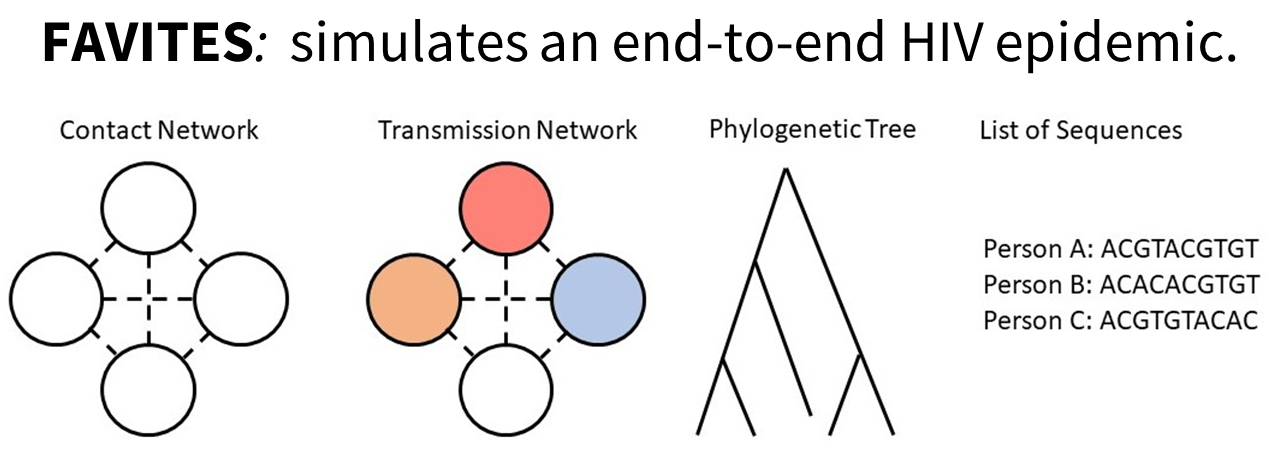
\includegraphics[scale=0.3]{Figures/FAVITES.png}
\caption{FAVITES simulates and end-to-end epidemic.}
\end{figure}

To measure the efficacy of each evaluative tool and their results to the environmental conditions we use six distinct metrics to generate optimal orderings. Each metric defines a unique way of calculating the count values for individuals, such that individuals with higher count values will have higher priority in the ordering. The resulting optimal ordering is then compared to the ordering produced by the prioritization algorithm given the simulated viral sequences as an input. 

The optimal ordering is a list of individuals who are at greatest risk of transmitting HIV. Individuals who transmit HIV more often and more frequently than other individuals are those that should be prioritized the highest, thus an optimal ordering is one which prioritizes these people the most. The count values generated by each metric are a way to calculate the priority of an individual based on different factors, such as the frequency they have transmitted HIV to others, which is then sorted into the ordering.

The Kendall Tau-b correlation coefficient is calculated with a variety of orderings generated by our metrics for given algorithms. The framework can provide a greater understanding of how optimal a particular ordering is by comparing an algorithm's ordering of individuals to the optimal ordering for a given metric. The following are our metrics for calculating count values of our optimal orderings:
\newline\newline
%LIST OF METHODS-------------------------------------------------
\begin{itemize}

\item \textbf{Metric 1: Direct Transmissions} This metric examines the direct impact an individual has on the spread of HIV within a population by assigning each individual a count value representing the total number of individuals they directly transmitted HIV to. Representing the individual with HIV as the red node, the direct transmissions of the red node would be all the yellow nodes (\textit{Figure 3}).\newline\newline

\item \textbf{Metric 2: Transmission Rate} This metric aims to represent each individual's rate of HIV transmission, taking into account that individuals who transmitted HIV to others recently should have higher priority than individuals have not transmitted HIV recently. Thus, if two different individuals have a high number of direct transmissions, if one individual made most of their transmissions years ago, and the other made their transmissions recently, the latter one ought to be prioritized.

Each individual's count is calculated as the slope of a linear regression  plotted over a step graph including all of the individual's outgoing transmissions over time (\textit{Figure 2}). The first point is placed at the time of the individual's first outgoing transmission. Thus, an individual that transmitted HIV to the most individuals over a short time period will have the steepest slope. Additionally, individuals who transmitted HIV more recently than others will have a greater positive slope and will be prioritized higher. 
\newline\newline

%------FIGURE 3
\begin{figure}[h!]
\centering
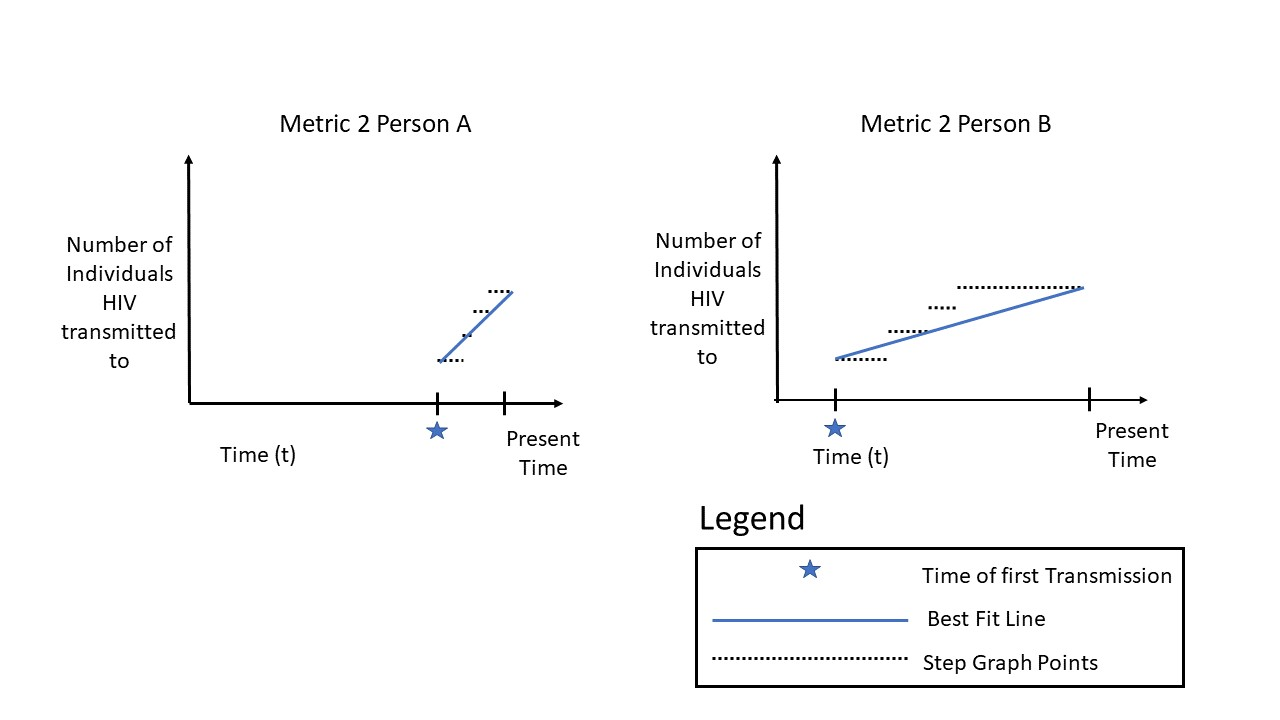
\includegraphics[scale=0.39]{Figures/Metric 2.jpg}
\caption{Above, we illustrate example plots for two individuals, where one  individual transmitted HIV to others more recently (\textit{2a}) and the other individual transmitted HIV others longer ago (\textit{2b}), with the graph on the left having a greater slope and thus representing an individual with greater priority.}
\end{figure}
%------FIGURE 3 END
\item \textbf{Metric 3: Indirect Transmissions} This metric extends Metric 1 in order to analyze an individual's greater effect on the community. 

Each individual's count is calculated as the number of individuals they indirectly transmitted HIV to. More specifically, we count the number of individuals that HIV was directly transmitted to by this the partners that this individual transmitted HIV to. (\textit{Figure 3}). \newline\newline

\item \textbf{Metric 4: Total Transmissions} This metric merges Metrics 1 and 3 by taking into account both an individual's direct and indirect transmissions. 

Each individual's count is calculated as the sum of the number of partners that they directly transmitted HIV to and the number of individuals that those partners transmitted HIV to.
\newline\newline

\item \textbf{Metric 5: Number of Contacts} Here, we assign counts as the individual's total number of contacts, where a contact is someone who the individual in question has interacted with in a way that could transmit HIV, regardless of the individuals' actual HIV status. The goal of this metric is to account for the total number of partners an individual has.
\newline\newline

\item \textbf{Metric 6: Number of Contacts and Transmissions} In this metric, we merged Metric 1 and Metric 5, such that we examine each individual's direct number of transmissions and their total number of contacts. Thus, the count for each individual is the sum of their number of direct transmissions and their total number of contacts.\newline\newline

\end{itemize}

%------FIGURE 4
\begin{figure}[h!]
\centering
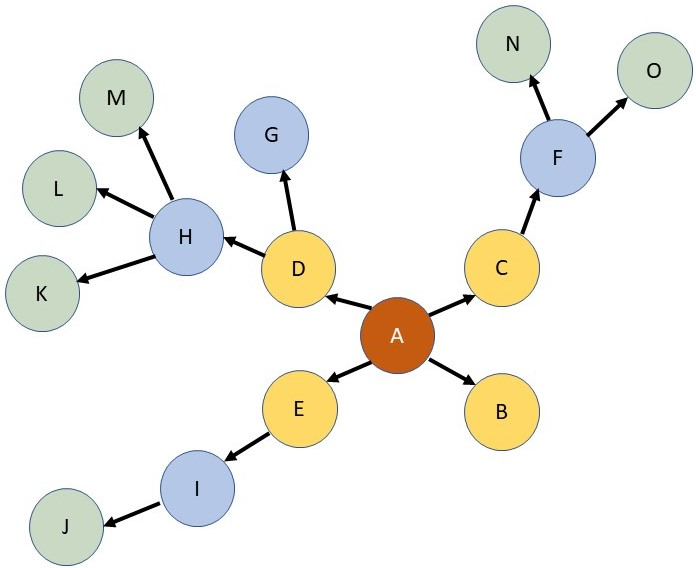
\includegraphics[scale=0.67]{Figures/transmission network.jpg}
\caption{An illustration of how individuals are counted in Metric 1, Metric 3, and Metric 4.
Let every node in the graph represent an HIV positive individual, with the red node representing the individual \textit{H} we are calculating a count value for, and let every directed edge between nodes represent a transmission of HIV from one individual to another.
To calculate the count for \textit{H}, \textbf{Metric 1} would count all orange nodes.
\textbf{Metric 3} would count all blue nodes, while \textbf{Metric 4} merges these two metrics by counting all orange nodes \textit{and} all blue nodes.} 
\end{figure}
%------FIGURE 4 END


%END LIST OF METHODS-----------------------------------------------------

In the final step of all six of our metrics, the list of individuals' counts are sorted in descending order of priority is compared to the ordering outputted by the prioritization algorithm \textit{X}. This comparison is done by calculating the Kendall Tau-b correlation coefficient between these two lists. This coefficient describes how closely-related the solution's ordering is to the most optimal (sorted) ordering \cite{kendall1938new}. A value of 1.0 indicates perfect correlation, or greatest possible accuracy, and a value of 0 indicates no correlation, or an accuracy no better than a  randomly selected ordering.

$Redundant to say we ran on HIV-Trace and ProACT again as we already said it above$
\section*{Results}
We tested SEPIA on two algorithms, HIV-Trace and ProACT, which have different approaches to determining individual priorities \cite{wertheim2018growth, moshiri2019ProACT}. Figure 4 shows the combined results of all 6 metrics. Figures 5 through Figure 10 represent the results of ProACT and HIV-Trace on Metrics 1 through Metric 6 respectively. These figures show the results of running ProACT and HIV-Trace on SEPIA using simulated data from FAVITES many different data sets under different conditions. 

\begin{figure}[h!]  %Figure 5
\centering
\title\textbf{Metric Results On ProACT and HIV-Trace}\par\medskip
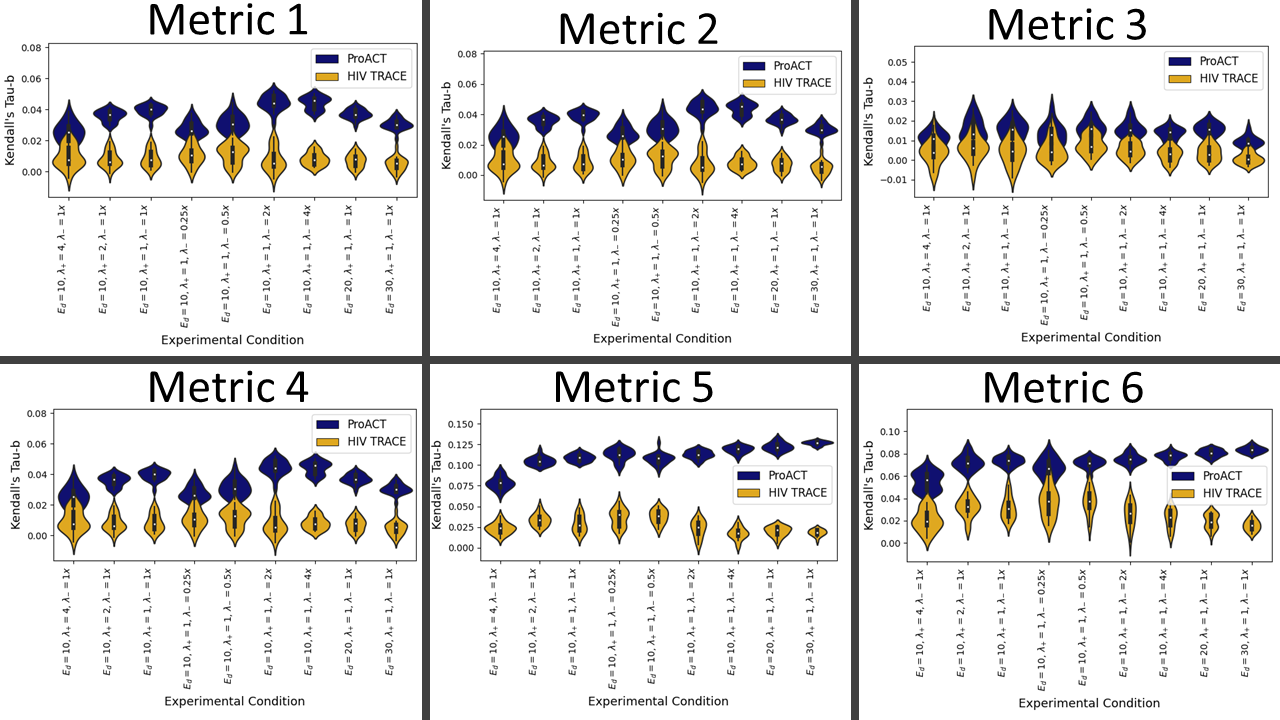
\includegraphics[scale=0.365]{Figures/all_metrics.png}
\caption{The results of all six metrics in SEPIA when comparing the orderings of Pro-ACT and HIV-Trace to the optimal ordering generated by the metrics of SEPIA.} 
\end{figure}

\begin{figure}[h!]  %Figure 6
\centering
\title\textbf{Metric 1}\par\medskip
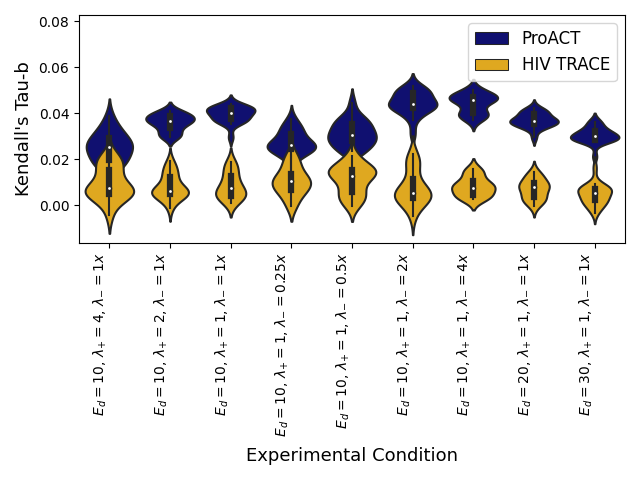
\includegraphics[scale=0.7]{Figures/m1_tau.png}
\caption{Metric 1: A violin plot showing the results of SEPIA on HIV-Trace and ProACT over simulated data with different conditions. All conditions receive a correlation coefficient above, but still close to, zero. Thus, it shows that both algorithms create orderings which are close to random compared to the optimal ordering generated by the metric. \cite{wertheim2018growth, moshiri2019ProACT}.} 
\end{figure}

\begin{figure}[h!]  %Figure 7
\centering
\title\textbf{Metric 2}\par\medskip
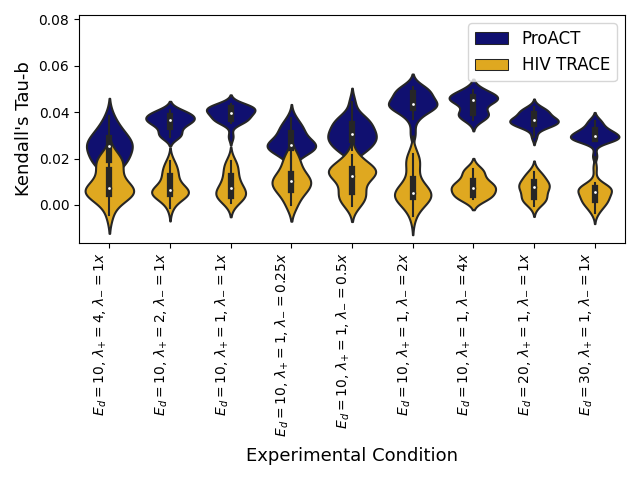
\includegraphics[scale=0.7]{Figures/m2_tau.png}
\caption{Metric 2: A violin plot showing the results of SEPIA on HIV-Trace and ProACT over simulated data with different conditions. All conditions receive a correlation coefficient above, but still close to, zero. Thus, it shows that both algorithms create orderings which are close to random compared to the optimal ordering generated by the metric. \cite{wertheim2018growth, moshiri2019ProACT}.} 
\end{figure}

\begin{figure}[h!] %Figure 8
\centering
\title\textbf{Metric 3}\par\medskip
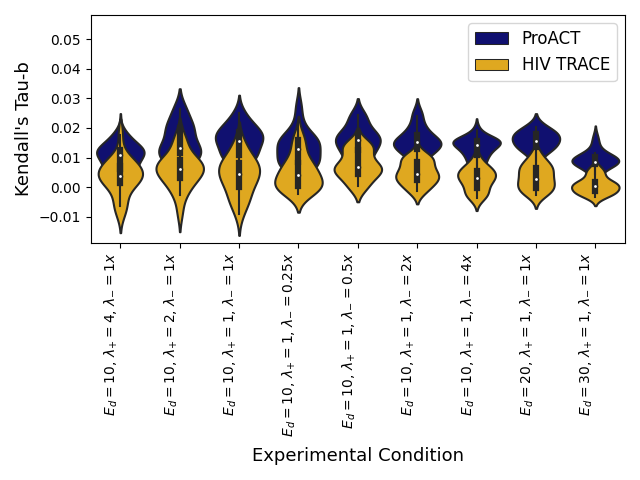
\includegraphics[scale=0.7]{Figures/m3_tau.png}
\caption{Metric 3: A violin plot showing the results of SEPIA on HIV-Trace and ProACT over simulated data with different conditions. All conditions receive a correlation coefficient above, but still close to, zero. Thus, it shows that both algorithms create orderings which are close to random compared to the optimal ordering generated by the metric. \cite{wertheim2018growth, moshiri2019ProACT}.} 
\end{figure}

\begin{figure}[h!] %Figure 9
\centering
\title\textbf{Metric 4}\par\medskip
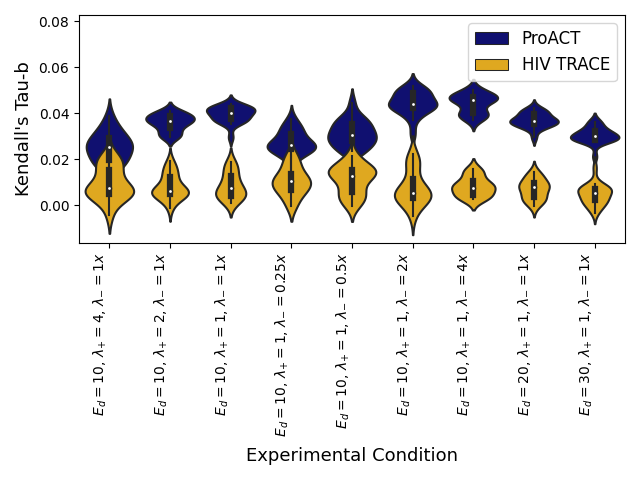
\includegraphics[scale=0.7]{Figures/m4_tau.png}
\caption{Metric 4: A violin plot showing the results of SEPIA on HIV-Trace and ProACT over simulated data with different conditions. All conditions receive a correlation coefficient above, but still close to, zero. Thus, it shows that both algorithms create orderings which are close to random compared to the optimal ordering generated by the metric. \cite{wertheim2018growth, moshiri2019ProACT}.} 
\end{figure}

\begin{figure}[h!] %Figure 10
\centering
\title\textbf{Metric 5}\par\medskip
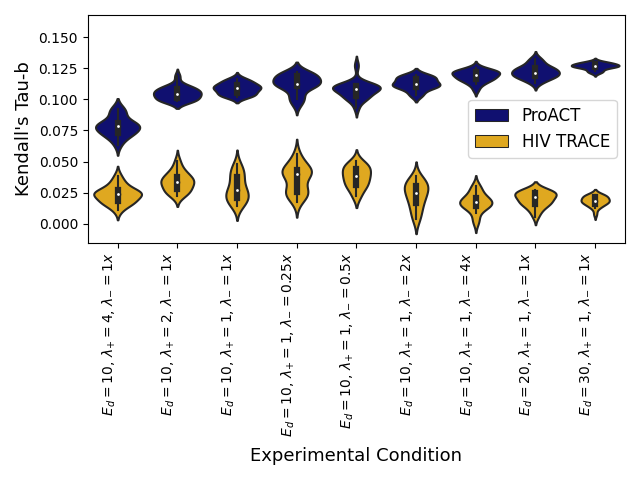
\includegraphics[scale=0.7]{Figures/m5_tau.png}
\caption{Metric 5: A violin plot showing the results of SEPIA on HIV-Trace and ProACT over simulated data with different conditions. All conditions receive a correlation coefficient above, but still close to, zero. Thus, it shows that both algorithms create orderings which are close to random compared to the optimal ordering generated by the metric. \cite{wertheim2018growth, moshiri2019ProACT}.} 
\end{figure}

\begin{figure}[h!] %Figure 11
\centering
\title\textbf{Metric 6}\par\medskip
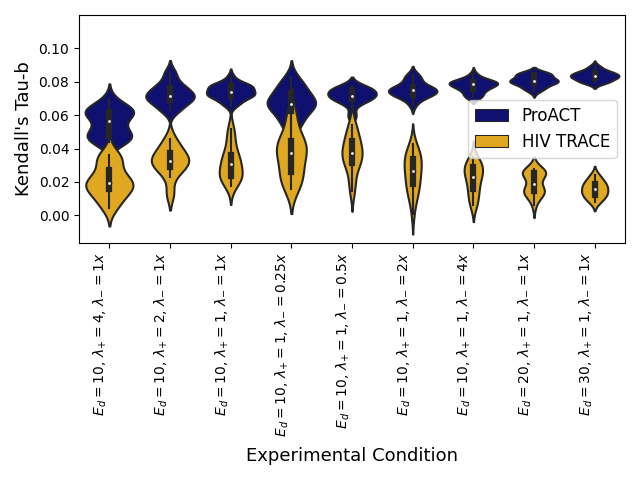
\includegraphics[scale=0.7]{Figures/m6_tau.png}
\caption{Metric 6: A violin plot showing the results of SEPIA on HIV-Trace and ProACT over simulated data with different conditions. All conditions receive a correlation coefficient above, but still close to, zero. Thus, it shows that both algorithms create orderings which are close to random compared to the optimal ordering generated by the metric. \cite{wertheim2018growth, moshiri2019ProACT}.} 
\end{figure}

\section*{Discussion}
Our results show that while ProACT does perform slightly better than HIV-Trace, neither model performs significantly better than random in predicting the next individual to become HIV positive in any environmental condition. Both these algorithms' Kendall Tau-b correlation coefficients are near 0.00 in all metrics, which means they perform little better than a random ordering in comparison to the optimal ordering of individuals who ought to be prioritized. Thus, there is low correlation between the order given by these algorithms and the optimal order generated by the metrics.

The metrics that both ProACT and HIV-Trace perform the best at relative to the others are on Metric 5 and Metric 6, albeit that both of these still have low correlation coefficients reaching around 0.100. 

The figures shows that the results of Metric 1 look very similar to the results of Metric 2. This is likely due to the dataset containing no individual with a significantly greater amount of transmissions in the given range of time. It is likely that if one individual has a high number of direct infections, their step count would also be very steep. Thus, Metric 2 in this case will act relatively similarly to Metric 1 in the sense it will just count the number of direct transmissions.

With our solution, researchers will have a means to provide quantifiable measurements of efficacy for their prioritization algorithms, and thus, will be able to optimize accordingly in a test-driven development process. Additionally, researchers can now compare the success of various algorithms against others to see how different implementations perform at predicting the transmission of HIV.

Due to the nature of how HIV spreads and that SEPIA was designed the HIV in mind, this tool is best used for HIV algorithms. However, we expect to span the accuracy testing to other viruses in future works.
%%%%%%%%%%%%%%%%%%%%%%%%%%%%%%%%%%%%%%%%%%%%%%
%%                                          %%
%% Backmatter begins here                   %%
%%                                          %%
%%%%%%%%%%%%%%%%%%%%%%%%%%%%%%%%%%%%%%%%%%%%%%

\begin{backmatter}

\section*{Competing interests}
  The authors declare that they have no competing interests.

\section*{Author's contributions}
    NM conceived and directed this project. All members wrote the code for this project. KA, TJ, ML, TN and MS composed this manuscript.
    
\section*{Acknowledgements}
  We would like to acknowledge the Early Research Scholars Program organized by Professor Christine Alvarado and Vignesh Gokul at the University of California San Diego for granting us the opportunity to work with Professor Moshiri on this project.
  
\section*{Availability of data and materials}
    The dataset supporting the conclusions of this article is available in the SEPIA repository, https://github.com/Moshiri-Lab/SEPIA.

\section*{Consent for publication}
    Not Applicable.
    
\section*{Ethics approval and consent to participate}
    Not Applicable.
    
\section*{Author Information}
    Department of Computer Science and Engineering, University of California San Diego, 9500 Gilman Drive, La Jolla, CA, 92093, USA
    \newline
    Kimberly Almaraz, Tyler Jang, McKenna Lewis, Titan Ngo, Miranda Song and Niema Moshiri
%%%%%%%%%%%%%%%%%%%%%%%%%%%%%%%%%%%%%%%%%%%%%%%%%%%%%%%%%%%%%
%%                  The Bibliography                       %%
%%                                                         %%
%%  Bmc_mathpys.bst  will be used to                       %%
%%  create a .BBL file for submission.                     %%
%%  After submission of the .TEX file,                     %%
%%  you will be prompted to submit your .BBL file.         %%
%%                                                         %%
%%                                                         %%
%%  Note that the displayed Bibliography will not          %%
%%  necessarily be rendered by Latex exactly as specified  %%
%%  in the online Instructions for Authors.                %%
%%                                                         %%
%%%%%%%%%%%%%%%%%%%%%%%%%%%%%%%%%%%%%%%%%%%%%%%%%%%%%%%%%%%%%

% if your bibliography is in bibtex format, use those commands:
\bibliographystyle{bmc-mathphys} % Style BST file (bmc-mathphys, vancouver, spbasic).
\bibliography{bmc_article}      % Bibliography file (usually '*.bib' )
% for author-year bibliography (bmc-mathphys or spbasic)
% a) write to bib file (bmc-mathphys only)
% @settings{label, options="nameyear"}
% b) uncomment next line
%\nocite{label}

% or include bibliography directly:
% \begin{thebibliography}
% \bibitem{b1}
% \end{thebibliography}

%%%%%%%%%%%%%%%%%%%%%%%%%%%%%%%%%%%
%%                               %%
%% Figures                       %%
%%                               %%
%% NB: this is for captions and  %%
%% Titles. All graphics must be  %%
%% submitted separately and NOT  %%
%% included in the Tex document  %%
%%                               %%
%%%%%%%%%%%%%%%%%%%%%%%%%%%%%%%%%%%

%%
%% Do not use \listoffigures as most will included as separate files
%%
%\section*{Figures}
%%  \begin{figure}[H]
%  \caption{\csentence{Sample figure title.}
%      A short description of the figure content
%      should go here.}
%      \end{figure}
%
%\begin{figure}[H]
%  \caption{\csentence{Sample figure title.}
%      Figure legend text.}
%      \end{figure}

%%%%%%%%%%%%%%%%%%%%%%%%%%%%%%%%%%%
%%                               %%
%% Tables                        %%
%%                               %%
%%%%%%%%%%%%%%%%%%%%%%%%%%%%%%%%%%%

%% Use of \listoftables is discouraged.
%%
%\section*{Tables}
%\begin{table}[H]
%\caption{Sample table title. This is where the description of the table should %go.}
%      \begin{tabular}{cccc}
%        \hline
%           & B1  &B2   & B3\\ \hline
%        A1 & 0.1 & 0.2 & 0.3\\
%        A2 & ... & ..  & .\\
%        A3 & ..  & .   & .\\ \hline
%      \end{tabular}
%%end{table}

%%%%%%%%%%%%%%%%%%%%%%%%%%%%%%%%%%%
%%                               %%
%% Additional Files              %%
%%                               %%
%%%%%%%%%%%%%%%%%%%%%%%%%%%%%%%%%%%
%%
%\section*{Additional Files}
%  \subsection*{Additional file 1 --- Sample additional file title}
%    Additional file descriptions text (including details of how to
%    view the file, if it is in a non-standard format or the file extension).  %This might
%    refer to a multi-page table or a figure.
%
%  \subsection*{Additional file 2 --- Sample additional file title}
%    Additional file descriptions text.


\end{backmatter}
\end{document}
